In order to explain our work and facilitate further implementations we have decided to show the logical flows aimed to create some features. The sequence diagrams will describe the interactions between the different parts of the system and the user.

\vspace{8mm}

\subsection{Login}
The ”Login” procedure starts when the user opens the app for the first time or whenever he logs out. The user can choose to be redirected to either Facebook or Google to complete the procedure. Immediately after logging on Facebook or Google the application will log into the Firebase Database. \\
Once this procedure is completed, the system will update the GUI by enabling the available sections.
In the event of an error, the system will show an error message.

\vspace{5mm}

\begin{figure}[h]
\centering
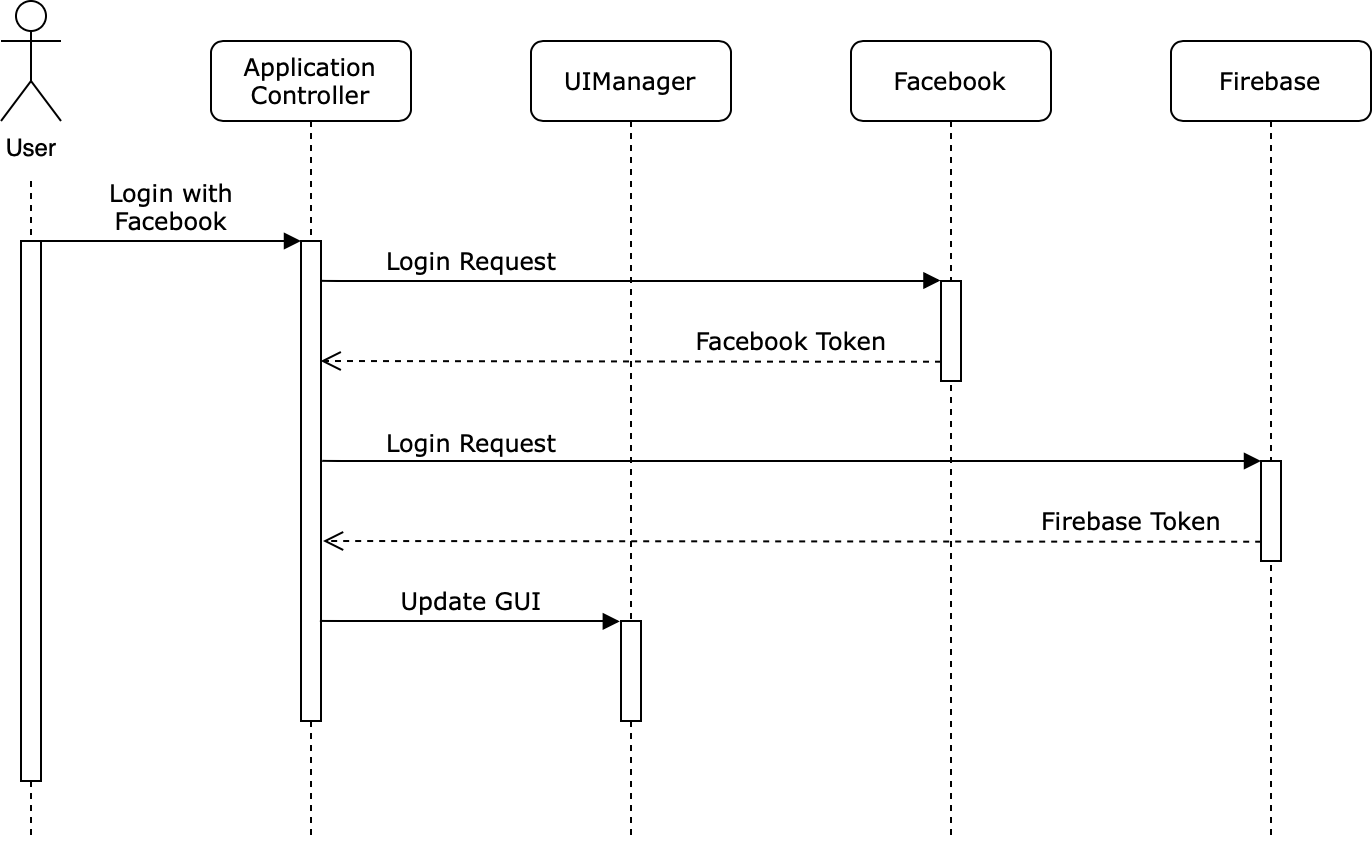
\includegraphics[scale=0.2]{img/seqdiagrams/loginfacebook}
\end{figure}

\begin{figure}[h]
\centering
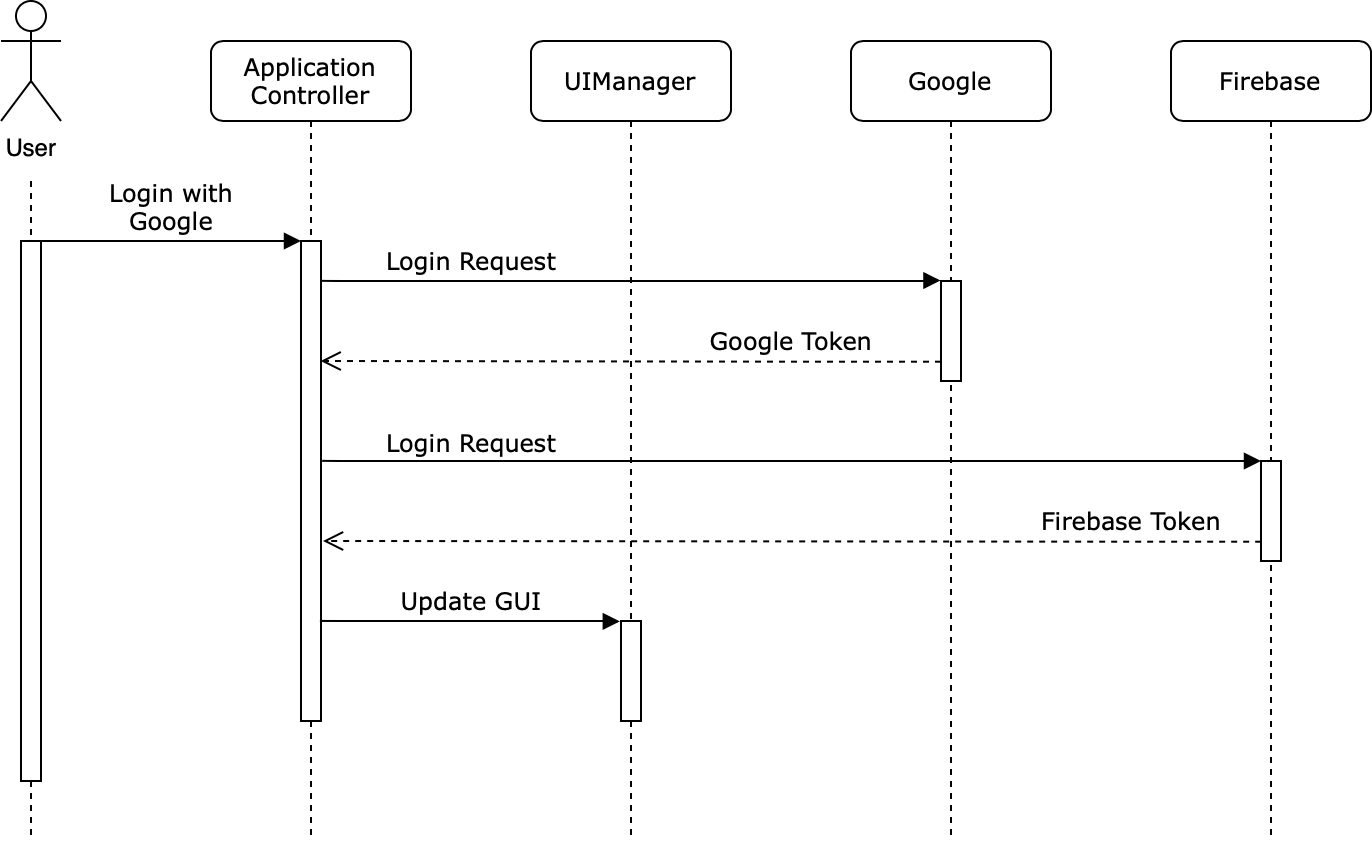
\includegraphics[scale=0.2]{img/seqdiagrams/logingoogle}
\end{figure}

\clearpage

\subsection{View Up Next}
The ”View Up Next” procedure starts when the user opens the application when he's already performed the login or when he presses the ”Up Next” tab in the Tab Bar. The sequence diagram shows the normal procedure. \\
After the user activates the "Up Next" tab, the application will send 3 requests to the ”MarvelAPI” service, one for each of the sections that will be displayed (comics released in the current week, comics released in the following week, comics released in the current month), in order to retrieve the titles of the issues belonging in each of the sections. \\
Once this information is obtained, the Controller will create a UITableViewCell for each issue and insert them into the correct section in a TableView. 

\vspace{5mm}

\begin{figure}[h]
\centering
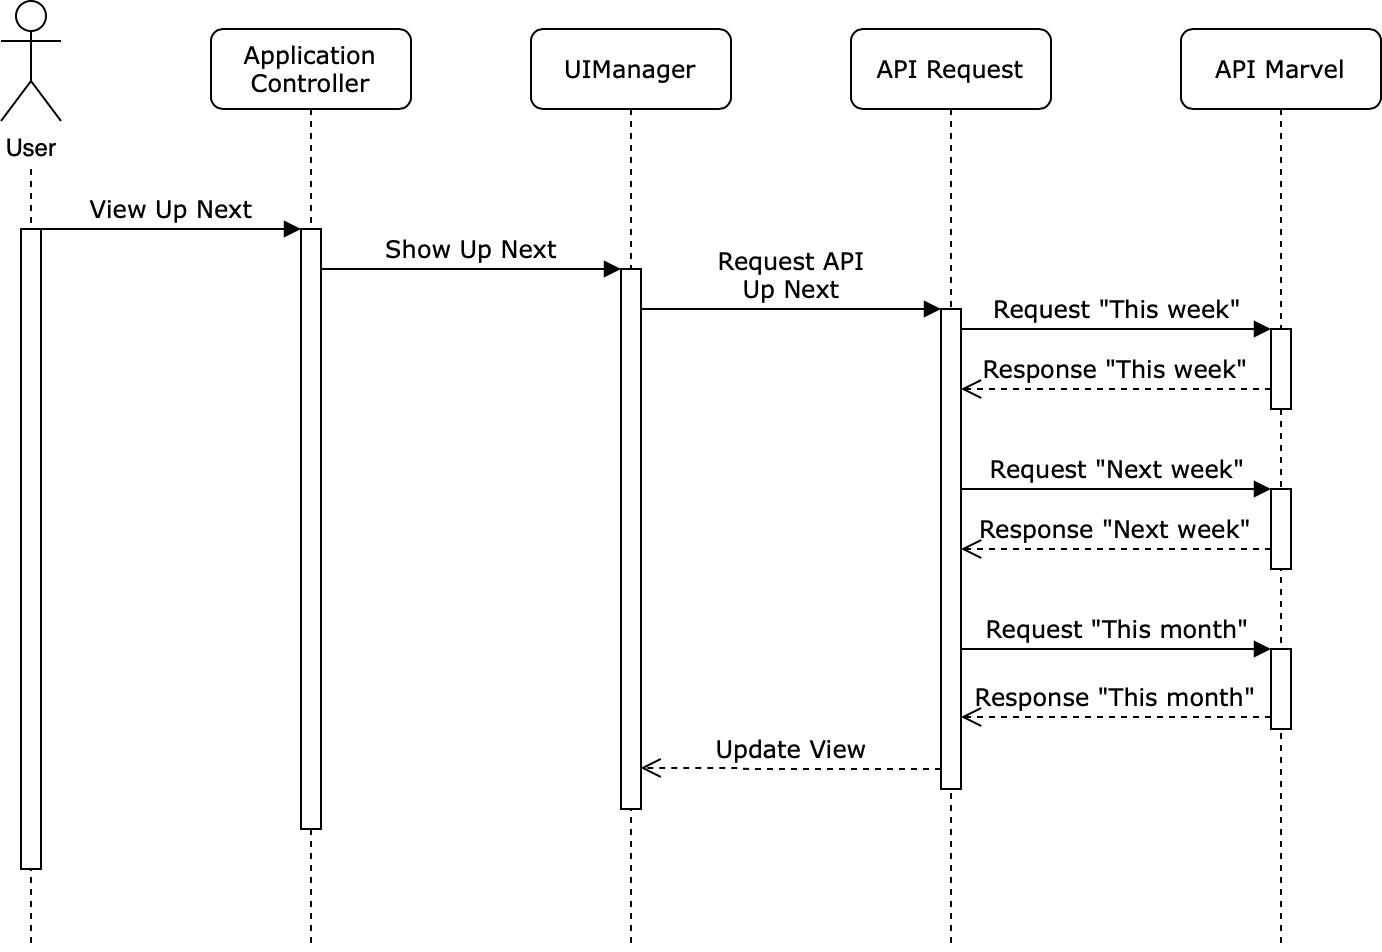
\includegraphics[width=\textwidth]{img/seqdiagrams/viewupnext}
\end{figure}

\clearpage

\subsection{View To Read}
The ”View To Read" procedure starts when the user presses the ”To Read” tab in the Tab Bar. The sequence diagram shows the normal procedure. \\
After the user activates the "To Read" tab, the application will send a request to Firebase in order to retrieve the identifiers of the next issues the user has to read. \\
Once these identifiers are obtained, the application will send a request to the "MarvelAPI" service in order to retrieve information about the issues. \\
Once this information is obtained, the Controller will create a custom UICollectionViewCell for each issue and insert them into a UICollectionView. \\
Furthermore and asynchronously, the application will download the cover of each issue to display to the user.

\vspace{5mm}

\begin{figure}[h]
\centering
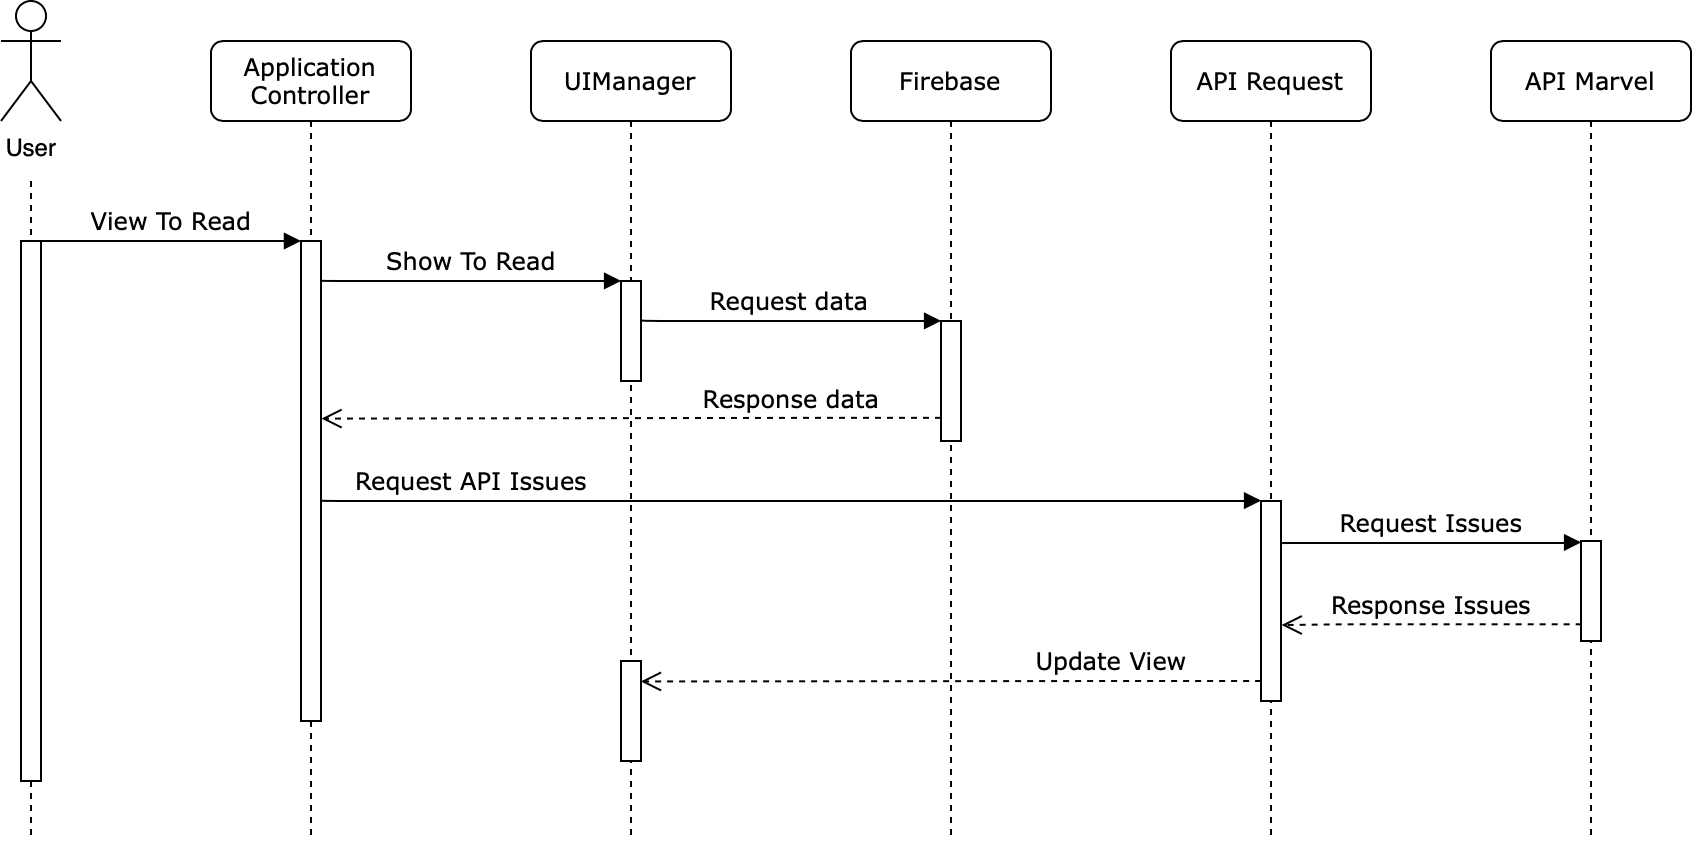
\includegraphics[width=\textwidth]{img/seqdiagrams/viewtoread}
\end{figure}

\clearpage

\subsection{View Issue}
The ”View Issue" procedure starts when the user presses a button representing an issue in one of the screens where such buttons are displayed. The sequence diagram shows the normal procedure. \\
After the user activates the "View Issue" button, the application will send a request to the "MarvelAPI" service in order to retrieve information about the issue. \\
Once this information is obtained, the Controller will create a set of UILabels, UITextViews and a UIImage to display the relevant information of the issue. 

\vspace{5mm}

\begin{figure}[h]
\centering
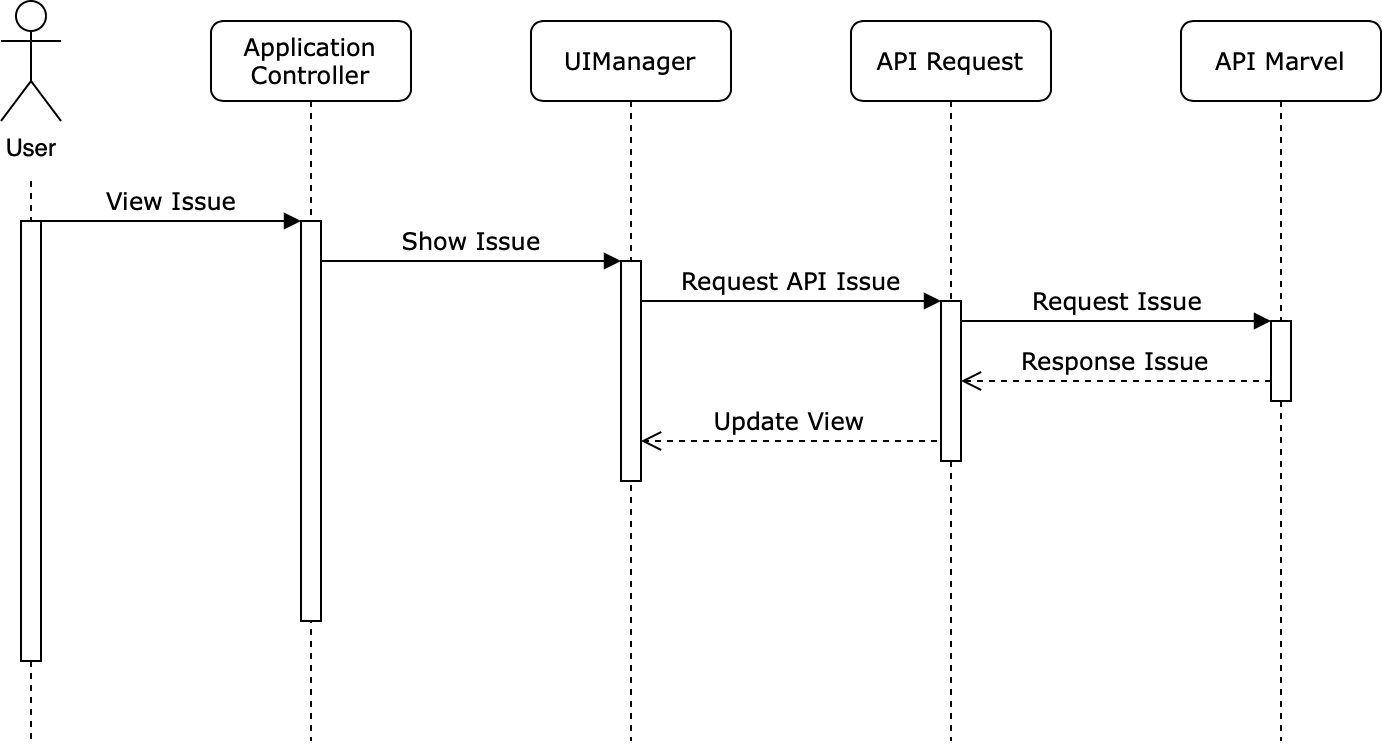
\includegraphics[width=\textwidth]{img/seqdiagrams/viewissue}
\end{figure}

\clearpage

\subsection{View Series}
The ”View Series" procedure starts when the user presses a button representing a series in one of the screens where such buttons are displayed. The sequence diagram shows the normal procedure. \\
After the user activates the "View Series" button, the application will send a request to the "MarvelAPI" service in order to retrieve information about the series. \\
Once all this information is obtained, the Controller will create a set of UILabels, UITextViews and a UIImage to display the relevant information of the series. 

\vspace{5mm}

\begin{figure}[h]
\centering
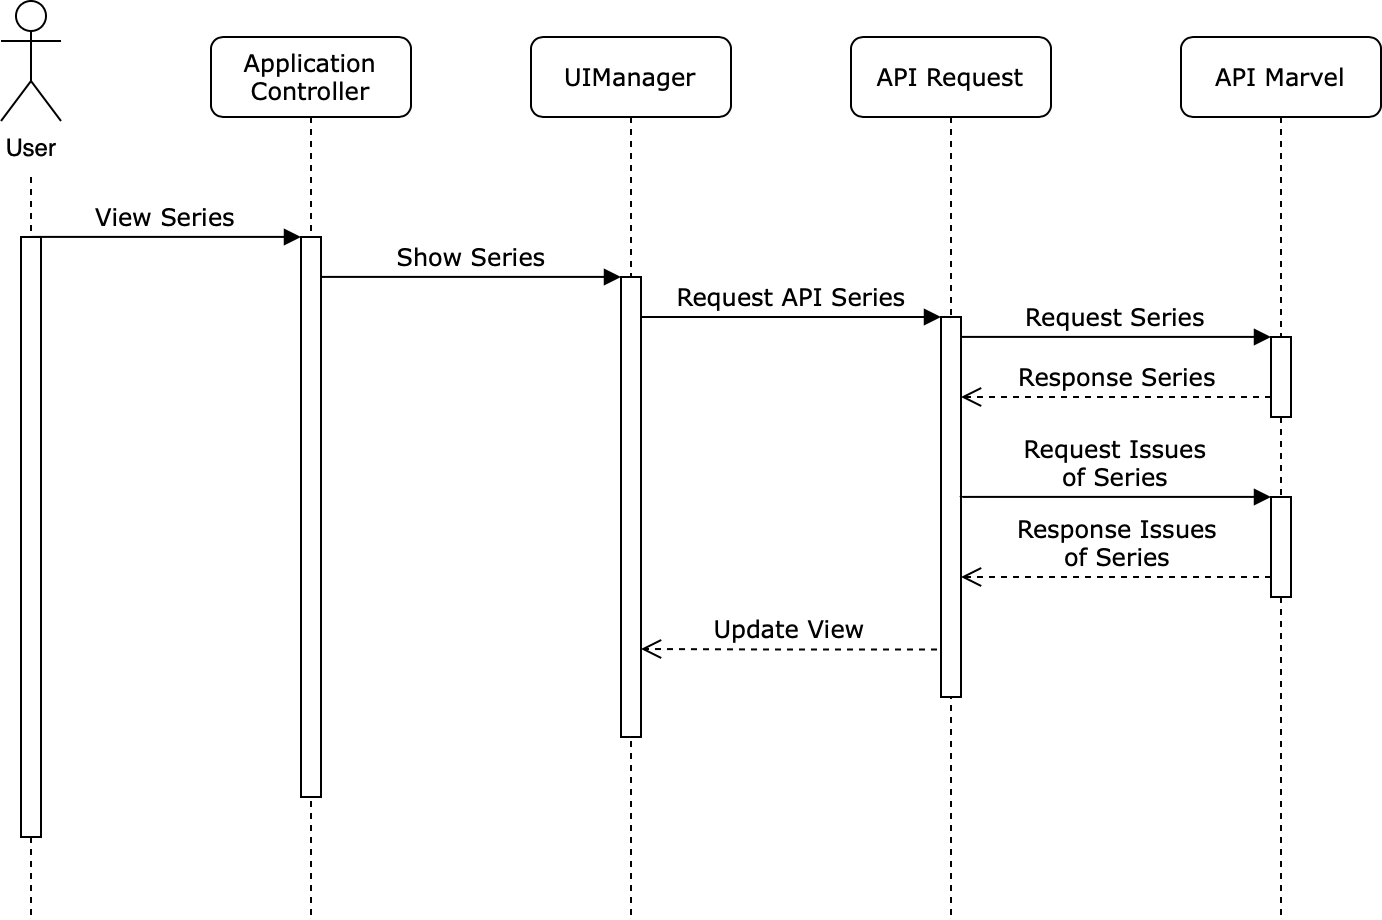
\includegraphics[width=\textwidth]{img/seqdiagrams/viewseries}
\end{figure}

\clearpage

\subsection{View Issues of Series}
The ”View Issues of Series" procedure starts when the user presses the "See all issues" button when he's viewing a series. The sequence diagram shows the normal procedure. \\
After the user activates the "See all issues" button, the application will send a request to the "MarvelAPI" service in order to retrieve all the issues belonging to that series. \\
Once all this information is obtained, the Controller will create a UITableViewCell for each issue and insert them into a UITableView, dividing them in expandable sections with 10 maximum cells for section. 

\vspace{5mm}

\begin{figure}[h]
\centering
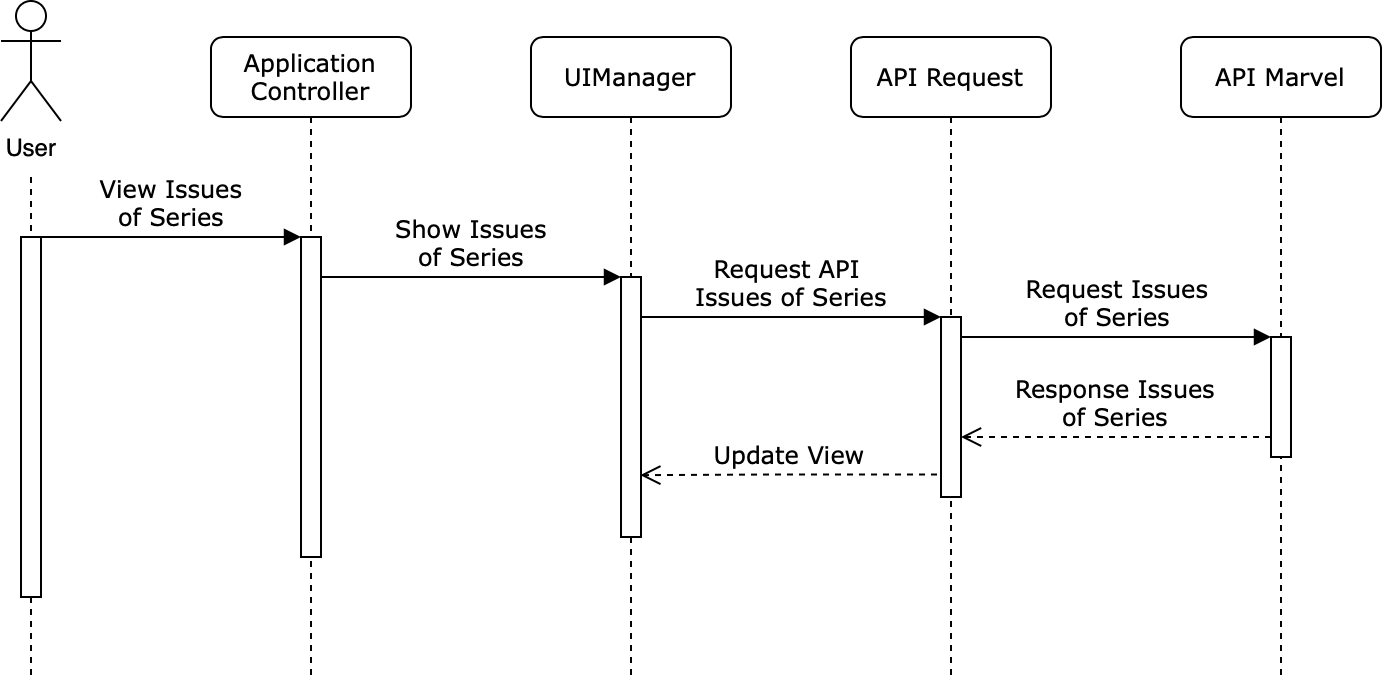
\includegraphics[width=\textwidth]{img/seqdiagrams/viewissuesofseries}
\end{figure}

\clearpage

\subsection{Mark Issue as Read}
The ”Mark Issue as Read" procedure starts when the user presses the corresponding button while he's either viewing an issue or the "To Read" section. The sequence diagram shows the normal procedure. \\
After the user activates the "Mark Issue as Read" button, the application will send a request to Firebase in order to register the issue as read in the database. \\
After receiving a notification of success, the Controller will update the GUI to show the success of the procedure. 

\vspace{5mm}

\begin{figure}[h]
\centering
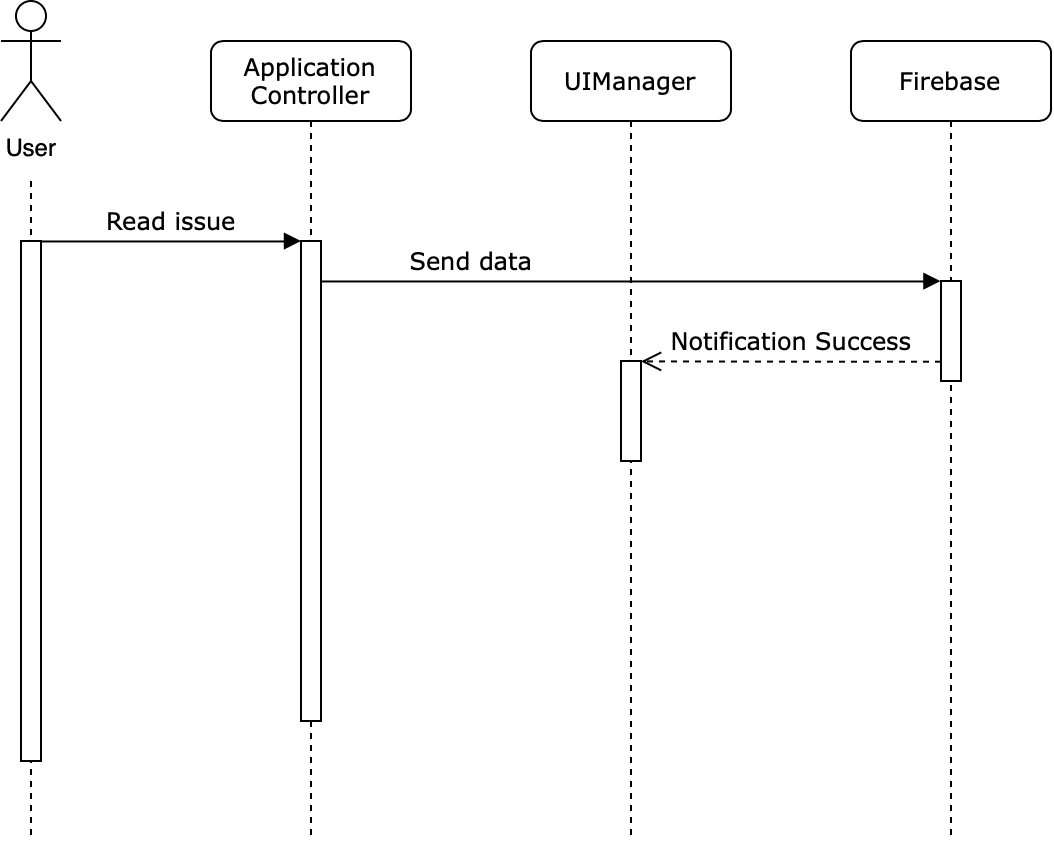
\includegraphics[width=\textwidth]{img/seqdiagrams/readissue}
\end{figure}

\clearpage

\subsection{Follow a Series}
The ”Follow a Series" procedure starts when the user presses the corresponding button while he's viewing a series. The sequence diagram shows the normal procedure. \\
After the user activates the "Follow a Series" button, the application will send a request to Firebase in order to register the series as followed in the database. \\
After receiving a notification of success, the Controller will update the GUI to show the success of the procedure. 

\vspace{5mm}

\begin{figure}[h]
\centering
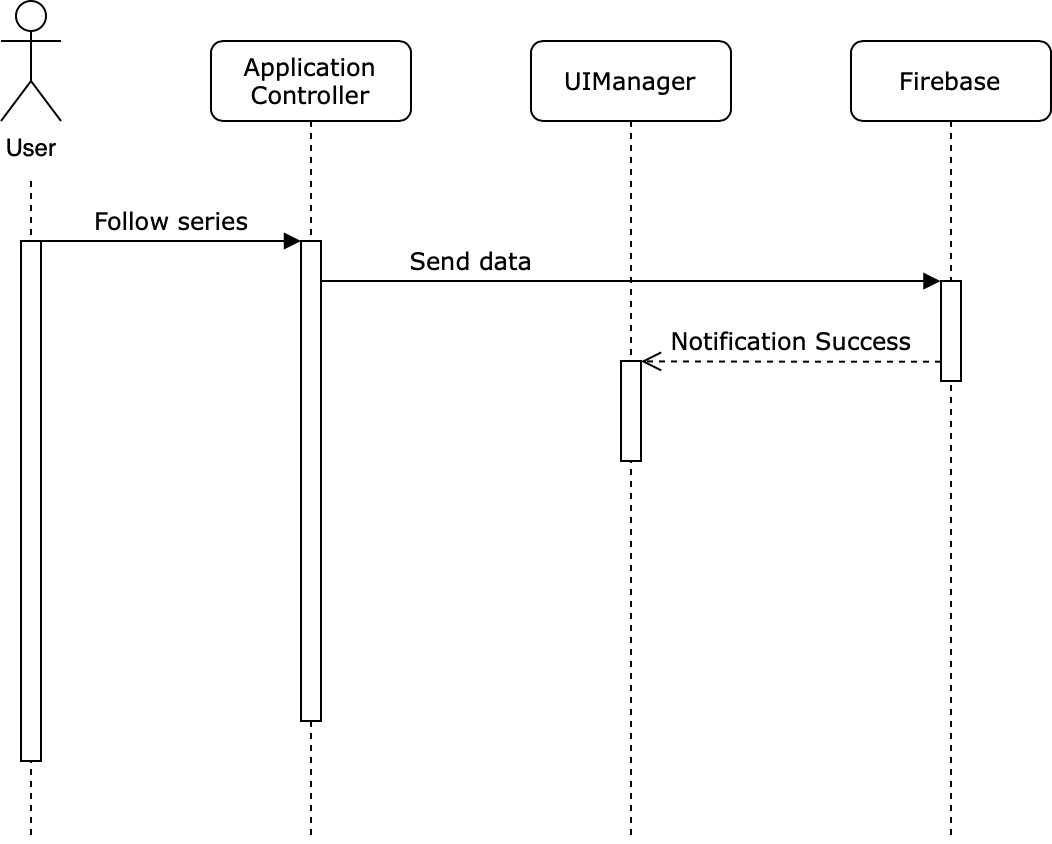
\includegraphics[width=\textwidth]{img/seqdiagrams/followseries}
\end{figure}

\clearpage

\subsection{Search for a Series}
The ”Search for a Series” procedure starts when the user presses the ”Search" tab in the Tab Bar. The sequence diagram shows the normal procedure. \\
After the user activates the "Search" tab, the application will send a request to the ”MarvelAPI” service in order to retrieve the series whose name matches the string written by the user. \\
Once this information is obtained, the Controller will create a UITableViewCell for each issue and insert them in a TableView. 

\vspace{5mm}

\begin{figure}[h]
\centering
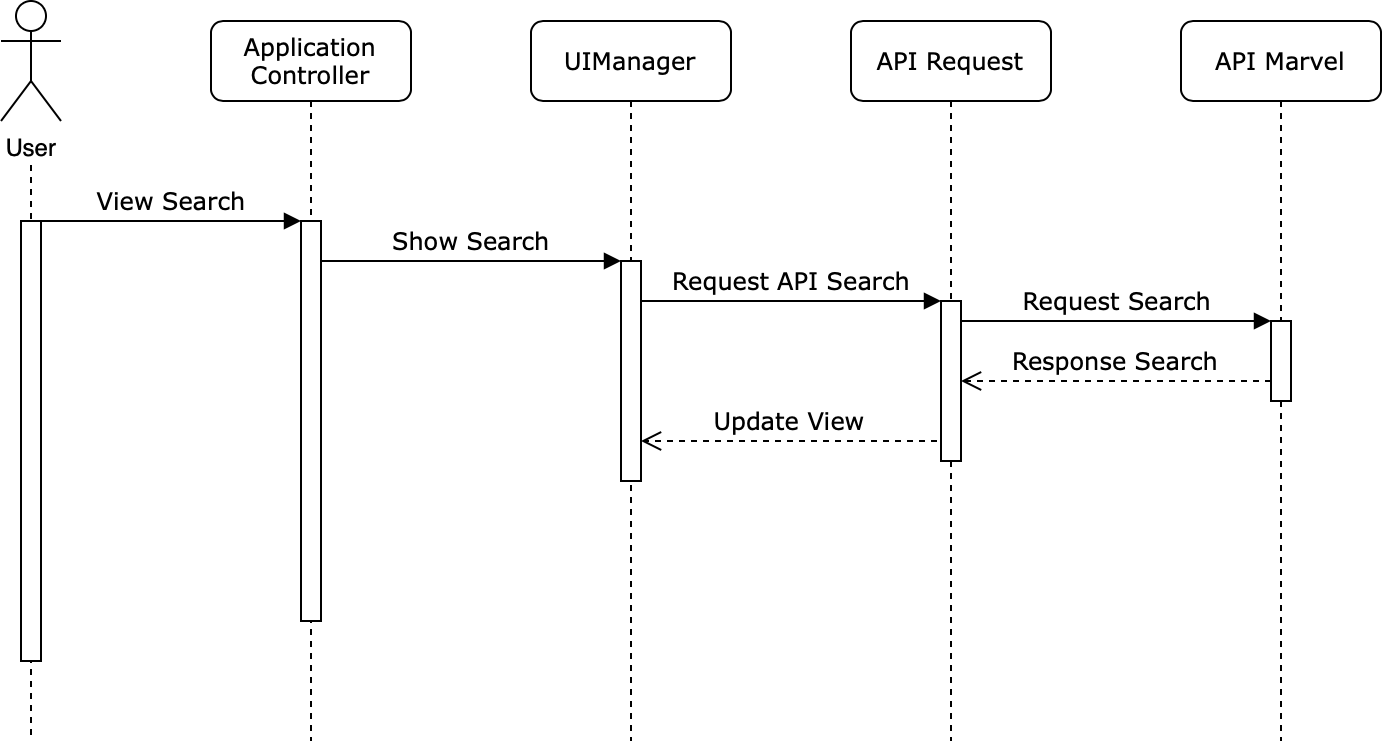
\includegraphics[width=\textwidth]{img/seqdiagrams/searchseries}
\end{figure}


